%! Author = TiagoRG
%! GitHub = https://github.com/TiagoRG

\documentclass{report}
\usepackage[T1]{fontenc} % Fontes T1
\usepackage[utf8]{inputenc} % Input UTF8
\usepackage[backend=biber, style=ieee]{biblatex} % para usar bibliografia
\usepackage{csquotes}
\usepackage[portuguese]{babel} %Usar língua portuguesa
\usepackage{blindtext} % Gerar texto automaticamente
\usepackage[dvipsnames]{xcolor}
\usepackage[printonlyused]{acronym}
\usepackage{hyperref} % para autoref
\usepackage{graphicx}
\usepackage{indentfirst}
\usepackage{float}
\usepackage{fancyhdr}
\usepackage{geometry}
\usepackage{listings}
\renewcommand{\familydefault}{\sfdefault}

\geometry{
    paper=a4paper,
    margin=45pt,
    % tmargin=70pt,
    includefoot
}

\lstset{
    language=C, % choose the language of the code
    basicstyle=\fontfamily{pcr}\selectfont\footnotesize\color{black},
    keywordstyle=\color{Blue}\bfseries, % style for keywords
    numbers=left, % where to put the line-numbers
    numberstyle=\tiny, % the size of the fonts that are used for the line-numbers
    backgroundcolor=\color{white},
    showspaces=false, % show spaces adding particular underscores
    showstringspaces=false, % underline spaces within strings
    showtabs=false, % show tabs within strings adding particular underscores
    frame=single, % adds a frame around the code
    tabsize=4, % sets default tabsize to 2 spaces
    rulesepcolor=\color{gray},
    rulecolor=\color{black},
    captionpos=b, % sets the caption-position to bottom
    breaklines=false, % sets automatic line breaking
    breakatwhitespace=false,
}

\bibliography{bibliography}


\begin{document}
%%
% Definições
\input{defs/definitions}
%
%%%%%% CAPA %%%%%%
%
\begin{titlepage}

\begin{center}
%
\vspace*{50mm}
%
{\Huge \titulo}\\
%
\vspace{10mm}
%
{\Large \empresa}\\
%
\vspace{10mm}
%
{\LARGE \autores}\\
%
\vspace{30mm}
%
\begin{figure}[h]
\center
\includegraphics{images/ua}\label{fig:ua-title-logo}
\end{figure}
%
\end{center}
\end{titlepage}

%%  Página de Título %%
\title{%
{\Huge\textbf{\titulo}}\\
\vspace*{1cm}
{\Large \departamento\\ \empresa}
}
%
\author{%
    \autores \\
    \autorescontactos
}
%
\date{\today}
%
\maketitle

%\pagenumbering{roman}

%%%%%% RESUMO %%%%%%
% \begin{abstract}
% Resumo de 200-300 palavras.
% \end{abstract}


%%%%%% Agradecimentos %%%%%%
%\renewcommand{\abstractname}{Agradecimentos}
%\begin{abstract}
    %Eventuais agradecimentos.
%\end{abstract}

\tableofcontents
%\listoftables     % descomentar se necessário
%\listoffigures    % descomentar se necessário


%%%%%%%%%%%%%%%%%%%%%%%%%%%%%%%
\clearpage

\renewcommand{\headrulewidth}{0pt}
\renewcommand{\footrulewidth}{0pt}
\fancypagestyle{plain}{
    \fancyhf{}% Clear header/footer
    % \fancyhead[R]{\small Universidade de Aveiro~~\includegraphics[width=20pt,height=20pt]{images/ua}}% Right header
    % \fancyhead[L]{\small Departamento de Electrónica, Telecomunicações e Informática}% Right header
    \fancyfoot[C]{\thepage}% Centred footer
}
\pagestyle{plain}% Set page style to plain.

%%%%%% INTRODUÇÃO %%%%%%
\input{ch/introducao}


%%%%%%%%%%%%%%%%%%%%%%%%%%%%%%%%

% Capítulos
\input{ch/imageblur}
\chapter{ImageMatchSubImage e ImageLocateSubImage}
\label{ch:imagematchlocatesubimage}
\section{Análise formal}
\label{sec:imagelocatesubimage/formal}

\section{Análise formal}
\label{sec:imagelocatesubimage/formal}

\input{sec/imagematchsubimage/formal.tex}

\subsection{ImageLocateSubImage}

\subsubsection{Descrição do algoritmo}

A função ImageLocateSubImage compara uma imagem (img2) com uma imagem maior (img1). Após as verificações iniciais, percorre-se cada pixel da imagem, comparando-o com o da subimagem. Se for detetado um pixel igual, chama-se a função ImageMatchSubImage para verificar se a subimagem está presente na imagem maior. No caso de encontrar um pixel que não corresponda, a função continua até encontrar, ou até acabar a imagem. Caso a ImageMatchSubImage devolva verdadeiro, a função devolve verdadeiro.

\subsubsection{Análise de complexidade}

\begin{itemize}
    
\item
\textbf{Complexidade Temporal}

Sabemos que ImageMatchSubImage, presente dentro do loop interior, é uma operação $O(p*o)$, e que se percorre a imagem linha a linha e coluna a coluna, logo é possível afirmar que a complexidade temporal do algoritmo é $O((n*m)*(p*o))$, onde n e m são a altura e largura de img2 e p e o são a altura e largura da subimagem verificada dentro do loop, respetivamente.

\item
\textbf{Complexidade Espacial}

A complexidade espacial do algoritmo é $O(1)$, dado que não são usadas estruturas de dados adicionais que cresçam com o tamanho da entrada. As variáveis row e col são as únicas variáveis adicionais, e ocupam um espaço constante.

\end{itemize}


\subsection{ImageLocateSubImage}

\subsubsection{Descrição do algoritmo}

A função ImageLocateSubImage compara uma imagem (img2) com uma imagem maior (img1). Após as verificações iniciais, percorre-se cada pixel da imagem, comparando-o com o da subimagem. Se for detetado um pixel igual, chama-se a função ImageMatchSubImage para verificar se a subimagem está presente na imagem maior. No caso de encontrar um pixel que não corresponda, a função continua até encontrar, ou até acabar a imagem. Caso a ImageMatchSubImage devolva verdadeiro, a função devolve verdadeiro.

\subsubsection{Análise de complexidade}

\begin{itemize}
    
\item
\textbf{Complexidade Temporal}

Sabemos que ImageMatchSubImage, presente dentro do loop interior, é uma operação $O(p*o)$, e que se percorre a imagem linha a linha e coluna a coluna, logo é possível afirmar que a complexidade temporal do algoritmo é $O((n*m)*(p*o))$, onde n e m são a altura e largura de img2 e p e o são a altura e largura da subimagem verificada dentro do loop, respetivamente.

\item
\textbf{Complexidade Espacial}

A complexidade espacial do algoritmo é $O(1)$, dado que não são usadas estruturas de dados adicionais que cresçam com o tamanho da entrada. As variáveis row e col são as únicas variáveis adicionais, e ocupam um espaço constante.

\end{itemize}

\section{Análise experimental}
\label{sec:imagelocatesubimage/experimental}

O gráfico seguinte foi gerado com a ajuda do \textit{LibreOffice Calc}. Para tal, foram primeiro gerados ficheiros, em formato csv, com os dados obtidos através da biblioteca \textit{time} da linguagem C. Depois foi gerado o gráfico a partir desse ficheiro, com resultados de 20 testes diferentes. Foi usado um computador com as seguintes especificações:

\begin{itemize}
    \item \textbf{CPU:} AMD Ryzen 7 5700U (16) @ 4.3GHz
    \item \textbf{GPU:} AMD Radeon RX Vega 8 [Lucienne]
    \item \textbf{RAM:} 16GB
\end{itemize}

\begin{figure}[H]
    \centering
    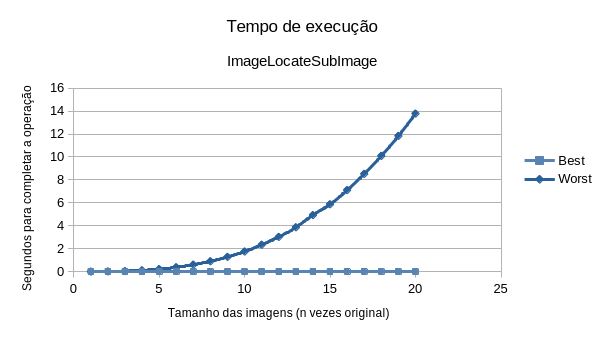
\includegraphics[width=\linewidth]{images/locatesubimage_chart.png}
    \caption{Gráfico do tempo de execução em função do tamanho das imagens fonte.}
    \label{fig:imageblur/locatesubimage_chart}
\end{figure}

Antes de fazer a análise do gráfico, é importante entender os valores. No eixo das abcissas está representado o tamanho das imagens fonte, ou seja, a imagem original, uma subimagem, e uma outra imagem que não pertence à imagem original. Para começar, a imagem original tem um tamanho de 300x300, a subimagem um tamanho de 50x50 (retirada do canto superior esquerdo da imagem original, de forma a obter o \textit{best case scenario}), e a outra imagem tem um tamanho de 100x100 (de forma a obter o \textit{worst case scenario}). Multiplica-se, então, o tamanho das imagens por cada um dos números de 2 a 20. No final, obtemos os tamanhos máximos de 6000x6000, 1000x1000 e 2000x2000, respetivamente. No eixo das ordenadas está representado o tempo de execução, em segundos, para os melhores e piores casos.

Como podemos ver na figura \ref{fig:imageblur/locatesubimage_chart}, o tempo de execução aumenta exponencialmente. Isto acontece porque o tempo de execução é proporcional ao tamanho das imagens fonte, logo se duplicarmos o tamanho de ambas as imagens, o tempo de execução passa a ser 8 vezes superior.

%%%%%% CONCLUSÕES %%%%%%
\input{ch/conclusao}

%%%%%% ACRÓNIMOS %%%%%%
%\input{defs/acronyms}


%%%%%%%%%%%%%%%%%%%%%%%%%%%%%%%%%
%\printbibheading
%\printbibliography

\input{ch/anexos}

\end{document}
